\documentclass[letter,11pt]{article}
%\documentclass[letter,twoside,11pt]{article}

\usepackage[spanish,es-nodecimaldot]{babel}
\usepackage[utf8]{inputenc}

\usepackage{lmodern}
\usepackage[T1]{fontenc}
\usepackage{textcomp}

\usepackage{graphicx}
\usepackage{pstricks}
\usepackage{enumitem}
\usepackage{longtable}

\usepackage{anysize}
\marginsize{3cm}{2cm}{2cm}{3cm}

\usepackage{amsmath}
\usepackage{array}
\usepackage{gensymb}
\usepackage{alltt}

\usepackage{fancyhdr}
\usepackage{lastpage}
\pagestyle{fancy}
\fancyhf{}
\fancyhead[LE,RO]{Laboratorio de Física Básica I}
\fancyfoot[CO,CE]{\thepage\ de \pageref{LastPage}}

\special{papersize=215.9mm,279.4mm}

\usepackage[
    pdfauthor={Carlos Eduardo Caballero Burgoa},%
    pdftitle={Laboratorio de Física Básica I},%
    pdfsubject={Movimiento con Aceleración Constante},%
    colorlinks,%
    citecolor=black,%
    filecolor=black,%
    linkcolor=black,%
    urlcolor=black,
    breaklinks]{hyperref}
\usepackage{breakurl}

\newcommand{\blankpage}{
\newpage
\thispagestyle{empty}
\mbox{}
\newpage
}

\renewcommand{\arraystretch}{1.2}

\begin{document}

\begin{titlepage}
\begin{center}
{\Large UNIVERSIDAD MAYOR DE SAN SIMÓN}\\
\vspace*{0.15cm}
{\large FACULTAD DE CIENCIAS Y TECNOLOGÍA}\\
\vspace*{0.10cm}
DEPARTAMENTO DE FÍSICA\\
\vspace*{3.0cm}
{\Large \textbf{LABORATORIO DE FÍSICA BÁSICA I}}\\
\vspace*{0.3cm}
{\Large \textbf{PRACTICA No. 6}}\\
\vspace*{3.5cm}
{\Large \textbf{MOVIMIENTO CON ACELERACIÓN CONSTANTE}}\\
\end{center}

\vspace*{7.4cm}
\leftskip=7.95cm
\noindent
\textbf{Estudiante:}\\
Caballero Burgoa, Carlos Eduardo.\\
\newline
\textbf{Docente:}\\
Msc. Guzmán Saavedra, Rocio.\\
\newline
\textbf{Grupo:} N5.\\
\textbf{Fecha de realización:} 30 de Diciembre del 2020.\\
\textbf{Fecha de entrega:} 31 de Diciembre del 2020.\\

\end{titlepage}

\blankpage

\section{Objetivo}
Determinar para un movimiento rectilíneo uniforme acelerado (MURA) las
relaciones funcionales:

\begin{enumerate}[label=(\alph*)]
    \item Posición en función del tiempo ($X$ vs $T$).
    \item Velocidad en función del tiempo ($V$ vs $T$).
    \item El valor de la aceleración.
\end{enumerate}

\section{Marco teórico}
La relación entre la posición y el tiempo de un móvil que se mueve sobre una
superficie horizontal, libre de rozamiento, con condición inicial $X_0=0$,
$V_0 = 0$ para $t_0=0$ es:

\begin{equation*}
    a = constante
\end{equation*}

\begin{equation*}
    a = \frac{dv}{dt}=\frac{d^2 x}{dt^2}
\end{equation*}

\begin{equation*}
    x = x_0 + v_0 t + \frac{1}{2} a t^2
\end{equation*}

\begin{equation}
    x = \frac{1}{2} a t^2
\end{equation}

La velocidad del móvil es:

\begin{equation*}
    a = \frac{dx}{dt}=a t
\end{equation*}
\begin{equation*}
    a = \frac{\Delta v}{\Delta t}=\frac{v_f-v_0}{t_f-t_0}
\end{equation*}

Para un $t_0=0$ obtenemos:

\begin{equation}
    v = v_0 + at
\end{equation}

\section{Materiales}
\begin{itemize}
\item Simulador «PHET cinemática».
\end{itemize}

\section{Procedimiento}
A continuación se describe el procedimiento experimental que se llevará a
cabo.

\begin{enumerate}
\item Haciendo uso del simulador, tomar datos de posición y velocidad en función
    del tiempo, establecidos el origen de partida y la velocidad inicial en
    cero, y una aceleración arbitraria.
\item Graficar los datos tomados tal que pueda verse la relación funcional entre
    estas variables.
\item Linealizar la curva de posición por el método de logaritmos.
\item Hallar la ecuación de la recta por el método gráfico.
\item Aplicar el método de mínimos cuadrados, para hallar los coeficientes de la
    recta y sus errores.
\item Determinar la aceleración a partir de los datos de posición y de
    velocidad.
\end{enumerate}

\section{Tablas de datos y resultados}

\subsubsection{Datos obtenidos ($a=3m/s^2$)}

\begin{center}
\begin{tabular}{|c|>{\centering}m{2.25cm}<{\centering}
                  |>{\centering}m{2.25cm}<{\centering}|}
\hline
\multicolumn{3}{|c|}{\textbf{Tabla \#1: Posición-Tiempo}} \\
\hline
$i$ & $t_i [s]$ & $x_i [m]$ \tabularnewline \hline
  1 & 0.0 &  0.00 \tabularnewline \hline
  2 & 0.1 &  0.01 \tabularnewline \hline
  3 & 0.2 &  0.04 \tabularnewline \hline
  4 & 0.3 &  0.09 \tabularnewline \hline
  5 & 0.3 &  0.17 \tabularnewline \hline
  6 & 0.4 &  0.26 \tabularnewline \hline
  7 & 0.5 &  0.37 \tabularnewline \hline
  8 & 0.6 &  0.51 \tabularnewline \hline
  9 & 0.7 &  0.67 \tabularnewline \hline
 10 & 0.8 &  0.84 \tabularnewline \hline
 11 & 0.8 &  1.04 \tabularnewline \hline
 12 & 0.9 &  1.26 \tabularnewline \hline
 13 & 1.0 &  1.50 \tabularnewline \hline
 14 & 1.1 &  1.76 \tabularnewline \hline
 15 & 1.2 &  2.04 \tabularnewline \hline
 16 & 1.3 &  2.34 \tabularnewline \hline
 17 & 1.3 &  2.67 \tabularnewline \hline
 18 & 1.4 &  3.01 \tabularnewline \hline
 19 & 1.5 &  3.37 \tabularnewline \hline
 20 & 1.6 &  3.76 \tabularnewline \hline
 21 & 1.7 &  4.17 \tabularnewline \hline
 22 & 1.8 &  4.59 \tabularnewline \hline
 23 & 1.8 &  5.04 \tabularnewline \hline
 24 & 1.9 &  5.51 \tabularnewline \hline
 25 & 2.0 &  6.00 \tabularnewline \hline
 26 & 2.1 &  6.51 \tabularnewline \hline
 27 & 2.2 &  7.04 \tabularnewline \hline
 28 & 2.3 &  7.59 \tabularnewline \hline
 29 & 2.3 &  8.17 \tabularnewline \hline
 30 & 2.4 &  8.76 \tabularnewline \hline
 31 & 2.5 &  9.37 \tabularnewline \hline
 32 & 2.6 & 10.00 \tabularnewline \hline
\end{tabular}
\quad
\begin{tabular}{|c|>{\centering}m{2.25cm}<{\centering}
                  |>{\centering}m{2.25cm}<{\centering}|}
\hline
\multicolumn{3}{|c|}{\textbf{Tabla \#2: Velocidad-Tiempo}} \\
\hline
$i$ & $t_i [s]$ & $v_i [m]$ \tabularnewline \hline
  1 & 0.0 & 0.00 \tabularnewline \hline
  2 & 0.1 & 0.25 \tabularnewline \hline
  3 & 0.2 & 0.50 \tabularnewline \hline
  4 & 0.3 & 0.75 \tabularnewline \hline
  5 & 0.3 & 1.00 \tabularnewline \hline
  6 & 0.4 & 1.25 \tabularnewline \hline
  7 & 0.5 & 1.50 \tabularnewline \hline
  8 & 0.6 & 1.75 \tabularnewline \hline
  9 & 0.7 & 2.00 \tabularnewline \hline
 10 & 0.8 & 2.25 \tabularnewline \hline
 11 & 0.8 & 2.50 \tabularnewline \hline
 12 & 0.9 & 2.75 \tabularnewline \hline
 13 & 1.0 & 3.00 \tabularnewline \hline
 14 & 1.1 & 3.25 \tabularnewline \hline
 15 & 1.2 & 3.50 \tabularnewline \hline
 16 & 1.3 & 3.75 \tabularnewline \hline
 17 & 1.3 & 4.00 \tabularnewline \hline
 18 & 1.4 & 4.25 \tabularnewline \hline
 19 & 1.5 & 4.50 \tabularnewline \hline
 20 & 1.6 & 4.75 \tabularnewline \hline
 21 & 1.7 & 5.00 \tabularnewline \hline
 22 & 1.8 & 5.25 \tabularnewline \hline
 23 & 1.8 & 5.50 \tabularnewline \hline
 24 & 1.9 & 5.75 \tabularnewline \hline
 25 & 2.0 & 6.00 \tabularnewline \hline
 26 & 2.1 & 6.25 \tabularnewline \hline
 27 & 2.2 & 6.50 \tabularnewline \hline
 28 & 2.3 & 6.75 \tabularnewline \hline
 29 & 2.3 & 7.00 \tabularnewline \hline
 30 & 2.4 & 7.25 \tabularnewline \hline
 31 & 2.5 & 7.50 \tabularnewline \hline
 32 & 2.6 & 7.75 \tabularnewline \hline
\end{tabular}
\end{center}

\section{Gráficas}

\subsection{Análisis posición-tiempo}
Para la tabla \#1 se tiene:

\begin{figure}[!h]
\centering
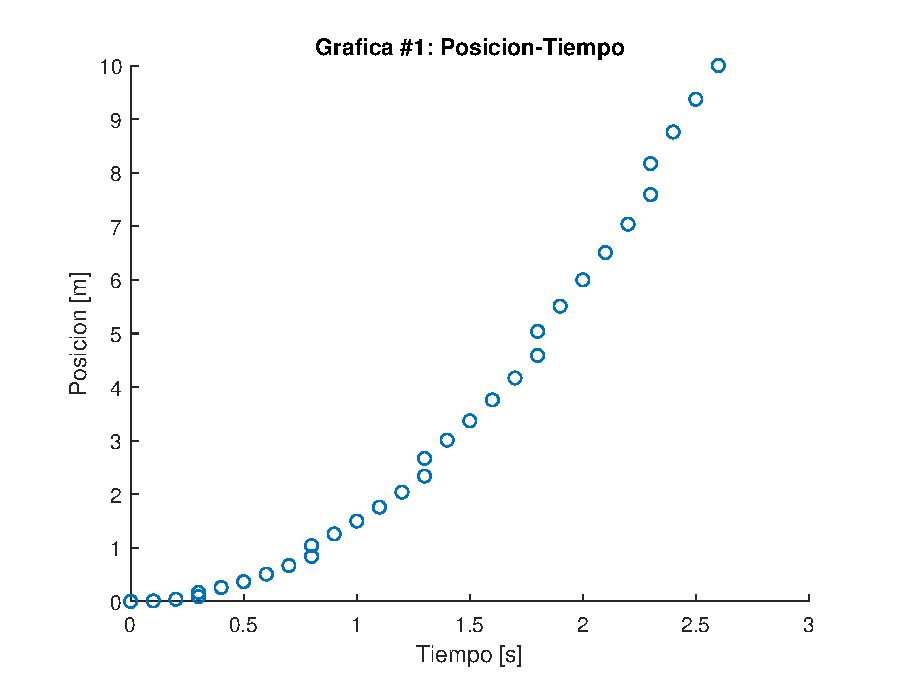
\includegraphics[scale=1.00]{resources/6.1.1.eps}
\caption{Gráfica de posición en función del tiempo}
\label{practica61}
\end{figure}

Por la forma de la figura \ref{practica61} el modelo que se asume para la
relación funcional $x = x(t)$ es:

\begin{equation}
    y = a x^b
\end{equation}

\subsubsection{Linealización por logaritmos}
Aplicando logaritmos a ambos lados de la ecuación, obtenemos:

\begin{equation*}
    \log y = \log a + b \log x
\end{equation*}

Haciendo los siguientes cambios de variables:

\begin{equation*}
    Y' = \log y
\end{equation*}
\begin{equation*}
    A = \log a
\end{equation*}
\begin{equation*}
    B = b
\end{equation*}
\begin{equation*}
    X' = \log x
\end{equation*}

Se obtiene:

\begin{equation*}
    Y' = A + B X'
\end{equation*}

\begin{center}
\begin{tabular}{|c|>{\centering}m{2.8cm}<{\centering}
                  |>{\centering}m{2.8cm}<{\centering}|}
\hline
$i$ & $\log(t_i)$ & $\log(x_i)$ \tabularnewline \hline
  1 & -       & -       \tabularnewline \hline
  2 & -1.0000 & -2.0000 \tabularnewline \hline
  3 & -0.6990 & -1.3979 \tabularnewline \hline
  4 & -0.5229 & -1.0458 \tabularnewline \hline
  5 & -0.5229 & -0.7696 \tabularnewline \hline
  6 & -0.3979 & -0.5850 \tabularnewline \hline
  7 & -0.3010 & -0.4318 \tabularnewline \hline
  8 & -0.2218 & -0.2924 \tabularnewline \hline
  9 & -0.1549 & -0.1739 \tabularnewline \hline
 10 & -0.0969 & -0.0757 \tabularnewline \hline
 11 & -0.0969 &  0.0170 \tabularnewline \hline
 12 & -0.0458 &  0.1004 \tabularnewline \hline
 13 &       0 &  0.1761 \tabularnewline \hline
 14 &  0.0414 &  0.2455 \tabularnewline \hline
 15 &  0.0792 &  0.3096 \tabularnewline \hline
 16 &  0.1139 &  0.3692 \tabularnewline \hline
 17 &  0.1139 &  0.4265 \tabularnewline \hline
 18 &  0.1461 &  0.4786 \tabularnewline \hline
 19 &  0.1761 &  0.5276 \tabularnewline \hline
 20 &  0.2041 &  0.5752 \tabularnewline \hline
 21 &  0.2304 &  0.6201 \tabularnewline \hline
 22 &  0.2553 &  0.6618 \tabularnewline \hline
 23 &  0.2553 &  0.7024 \tabularnewline \hline
 24 &  0.2788 &  0.7412 \tabularnewline \hline
 25 &  0.3010 &  0.7782 \tabularnewline \hline
 26 &  0.3222 &  0.8136 \tabularnewline \hline
 27 &  0.3424 &  0.8476 \tabularnewline \hline
 28 &  0.3617 &  0.8802 \tabularnewline \hline
 29 &  0.3617 &  0.9122 \tabularnewline \hline
 30 &  0.3802 &  0.9425 \tabularnewline \hline
 31 &  0.3979 &  0.9717 \tabularnewline \hline
 32 &  0.4150 &  1.0000 \tabularnewline \hline
\end{tabular}
\end{center}

La gráfica de los datos con el cambio de variable logarítmica pueden verse en la
figura \ref{practica62}.

\begin{figure}[!h]
\centering
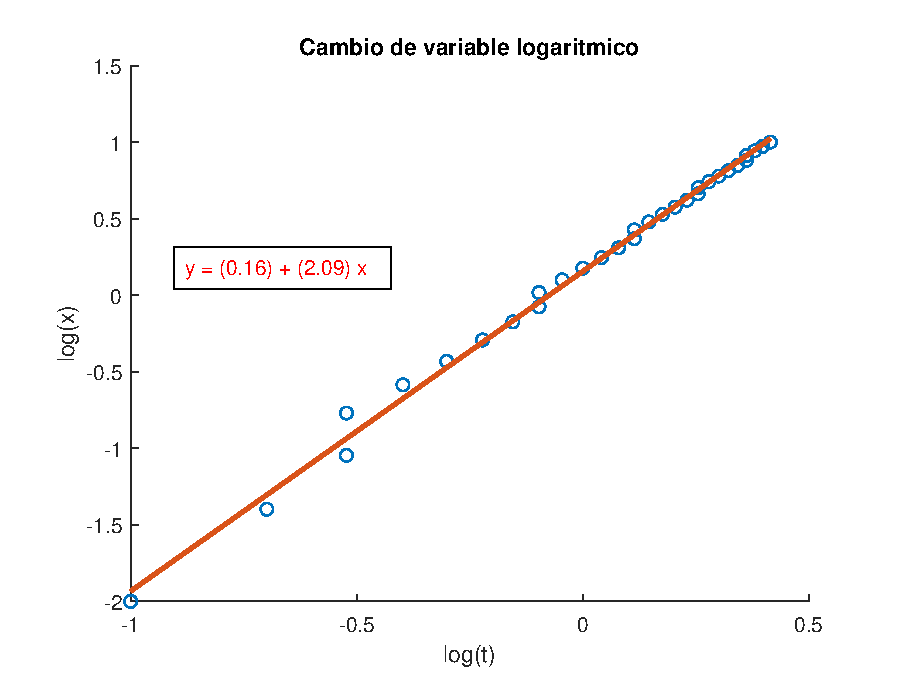
\includegraphics[scale=1.00]{resources/6.1.2.eps}
\caption{Gráfica linealizada por el método de logaritmos}
\label{practica62}
\end{figure}

\subsubsection{Método gráfico}
Calculando los parámetros $A$ y $B$:

\begin{equation*}
    A = 0.18
\end{equation*}

\begin{equation*}
    B = \frac{1.0+2.0}{0.4150+1.0} = \frac{3.0}{1.4150} = 2.12
\end{equation*}

La ecuación de la recta es:

\begin{equation*}
    Y' = 0.18 + 2.21 X'
\end{equation*}

A partir de los parámetros de recta $A$ y $B$, calculamos los parámetros $a$ y
$b$, de la curva:

\begin{equation*}
    a = antilog(A) = antilog(0.18) = 1.51
\end{equation*}
\begin{equation*}
    b = B = 2.21 \approx 2
\end{equation*}

La ecuación de la curva resultante es:

\begin{equation}
    y = 1.51 x^2
\end{equation}

\subsubsection{Memoria de calculo}

\paragraph{Entrada del programa}
\begin{alltt}
\footnotesize
\input{resources/i6_1.csv}
\normalsize
\end{alltt}

\paragraph{Comandos del programa}
\begin{alltt}
\footnotesize
\input{resources/p6_1_2.m}
\normalsize
\end{alltt}

\paragraph{Salida del programa}
\begin{alltt}
\footnotesize
\input{resources/o6_1_2.txt}
\normalsize
\end{alltt}

\subsubsection{Método analítico}
Calculando los valores de la recta por el método de los mínimos cuadrados, se
obtiene:

\begin{equation*}
    A = (0.156 \pm 0.009)[u];2.12\%
\end{equation*}

\begin{equation*}
    B = (2.09 \pm 0.02)[u];1.26\%
\end{equation*}

La ecuación de la recta es:

\begin{equation*}
    Y' = 0.156 + 2.09 X'
\end{equation*}

A partir de los parámetros de recta $A$ y $B$, calculamos los parámetros $a$ y
$b$, de la curva original y sus errores por el método de propagación de errores:

\begin{equation*}
    a = antilog(A) = antilog(0.156) = 1.43
\end{equation*}
\begin{equation*}
    b = B = 2.09
\end{equation*}
\begin{equation*}
    e_a = 10^A ln(10) e_A = 10^{(2.12)} ln(10) 0.009 = 0.03
\end{equation*}
\begin{equation*}
    e_b = e_B = 0.02
\end{equation*}

Obteniendo finalmente los valores de la curva:

\begin{equation*}
    a = (1.43 \pm 0.03)[u];2.12\%
\end{equation*}

\begin{equation*}
    b = (2.09 \pm 0.02)[u];1.26\%
\end{equation*}

La ecuación de la curva resultante es:

\begin{equation}
    y = 1.43 x^2
\end{equation}

\subsubsection{Memoria de calculo}

\paragraph{Entrada del programa}
\begin{alltt}
\footnotesize
\input{resources/i6_1.csv}
\normalsize
\end{alltt}

\paragraph{Comandos del programa}
\begin{alltt}
\footnotesize
\input{resources/p6_1_3.m}
\normalsize
\end{alltt}

\paragraph{Salida del programa}
\begin{alltt}
\footnotesize
\input{resources/o6_1_3.txt}
\normalsize
\end{alltt}

\subsubsection{Comparación de resultados}
Se obtuvieron los siguientes resultados:

\begin{center}
\begin{tabular}{|c|c|}
\hline
Método gráfico & $y = 1.51 x^2$ \\
\hline
Método analítico & $y = 1.43 x^2$ \\
\hline
\end{tabular}
\end{center}

Siendo el método gráfico, el mas próximo al resultado ideal $y = 1.5 x^2$.

\subsubsection{Calculo de la aceleración}
Para calcular la aceleración se necesitan reemplazar las variables siguientes:

\begin{equation*}
    A = \frac{1}{2} a
\end{equation*}

\begin{equation*}
    B = 2
\end{equation*}

Utilizando el resultado obtenido por el método gráfico, obtenemos:

\begin{equation}
    a = 2 * (1.51) = 3.02 [m/s^2]
\end{equation}

Utilizando el resultado obtenido por el método analítico, obtenemos el valor
representativo siguiente:

\begin{equation*}
    a = 2 * (1.43) = 2.86 [m/s^2]
\end{equation*}

y calculando el error por el método de propagación de errores:

\begin{equation*}
    e_a = 2 e_A = 2 (0.03) = 0.06
\end{equation*}

Finalmente obtenemos la aceleración:

\begin{equation}
    a = (2.86 \pm 0.06)[m/s^2];2.10\%
\end{equation}

\subsection{Análisis velocidad-tiempo}
Para la tabla \#2 se tiene:

\begin{figure}[!h]
\centering
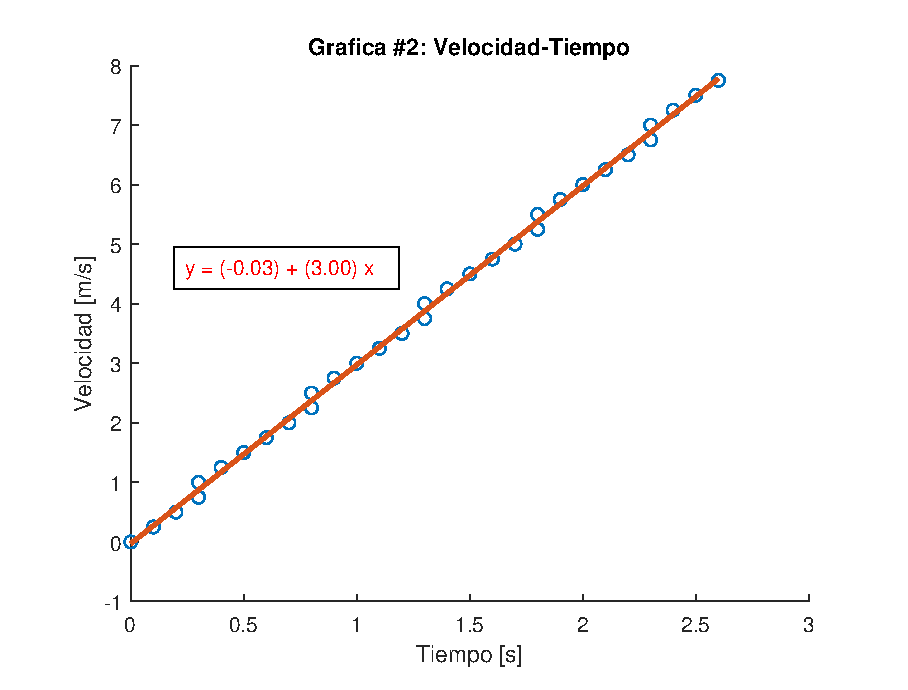
\includegraphics[scale=1.00]{resources/6.2.1.eps}
\caption{Gráfica de velocidad en función del tiempo}
\label{practica63}
\end{figure}

Por la forma de la figura \ref{practica63} el modelo que se asume para la
relación funcional $x = x(t)$ es:

\begin{equation*}
    v = A + B t
\end{equation*}

\subsubsection{Método gráfico}
Calculando los parámetros $A$ y $B$:

\begin{equation*}
    A = 0
\end{equation*}

\begin{equation*}
    B = \frac{7.75-0}{2.6-0} = \frac{7.75}{2.6} = 2.98
\end{equation*}

Por lo que la relación funcional $x = x(t)$ es:

\begin{equation}
    y = 2.98 x
\end{equation}

\subsubsection{Memoria de calculo}

\paragraph{Entrada del programa}
\begin{alltt}
\footnotesize
\input{resources/i6_2.csv}
\normalsize
\end{alltt}

\paragraph{Comandos del programa}
\begin{alltt}
\footnotesize
\input{resources/p6_2_1.m}
\normalsize
\end{alltt}

\paragraph{Salida del programa}
\begin{alltt}
\footnotesize
\input{resources/o6_2_1.txt}
\normalsize
\end{alltt}

\subsubsection{Método analítico}
Calculando los valores de la recta por el método de los mínimos cuadrados, se
obtiene:

\begin{equation*}
    A = (-0.03 \pm 0.03)[m];102.11\%
\end{equation*}

\begin{equation*}
    B = (3.00 \pm 0.02)[m/s];0.66\%
\end{equation*}

Siendo el coeficiente de correlación:
\begin{equation*}
    R = 0.9994
\end{equation*}

Con los parámetros obtenidos la relación $v = v(t)$ es:

\begin{equation}
    y = -0.03 + 3 x
\end{equation}

El significado físico de estos parámetros son que $A = -0.03$ es la velocidad
inicial $v_0$ cuando el tiempo es $0 [s]$, mientras que $B = 3.0$ representa la
aceleración constante con la que el objeto se desplaza.

\subsubsection{Memoria de calculo}

\paragraph{Entrada del programa}
\begin{alltt}
\footnotesize
\input{resources/i6_2.csv}
\normalsize
\end{alltt}

\paragraph{Comandos del programa}
\begin{alltt}
\footnotesize
\input{resources/p6_2_2.m}
\normalsize
\end{alltt}

\paragraph{Salida del programa}
\begin{alltt}
\footnotesize
\input{resources/o6_2_2.txt}
\normalsize
\end{alltt}

\subsubsection{Comparación de resultados}
Se obtuvieron los siguientes resultados:

\begin{center}
\begin{tabular}{|c|c|}
\hline
Método gráfico & $y = 2.98 x$ \\
\hline
Método analítico & $y = -0.03 + 3 x$ \\
\hline
\end{tabular}
\end{center}

Siendo el método analítico, el mas próximo al resultado ideal $y = 3.0 x$.

\subsubsection{Calculo de la aceleración}
Utilizando el resultado obtenido por el método gráfico, obtenemos:

\begin{equation}
    a = 2.98 [m/s^2]
\end{equation}

Utilizando el resultado obtenido por el método analítico, obtenemos el valor
representativo siguiente:

\begin{equation}
    a = (3.00 \pm 0.02)[m/s^2];0.66\%
\end{equation}

\subsection{Comparativa entre resultados}
Se obtuvieron los siguientes valores de la aceleración:

\begin{center}
\begin{tabular}{|c|c|}
\hline
\multicolumn{2}{|c|}{$x-t$} \\
\hline
Método gráfico & $a = 3.02 [m/s^2]$ \\
\hline
Método analítico & $a = (2.86 \pm 0.06)[m/s^2];2.10\%$ \\
\hline
\multicolumn{2}{|c|}{$v-t$} \\
\hline
Método gráfico & $a = 2.98 [m/s^2]$ \\
\hline
Método analítico & $a = (3.00 \pm 0.02)[m/s^2];0.66\%$ \\
\hline
\end{tabular}
\end{center}

Todos los resultados se aproximan al resultado ideal $a = 3$, con escasas
diferencias entre ellos, puede verse que calcular la aceleración a partir de las
mediciones de distancia crea mayor discrepancia, que el calculo de la
aceleración a partir de las mediciones de velocidad.

Probablemente estas diferencias se deban a la linealización de la curva y el
redondeo de los valores.

\end{document}
